\documentclass[border=2pt]{standalone}
\usepackage{tikz}
\usetikzlibrary{fadings}

\definecolor{Garnet}{rgb}{0.451,0.0,0.039}
\definecolor{Atlantic}{rgb}{0.275,0.416,0.624}
\definecolor{Congaree}{rgb}{0.122,0.255,0.302}
\definecolor{Horseshoe}{rgb}{0.396,0.471,0.043}
\definecolor{Rose}{rgb}{0.8,0.18,0.251}
\definecolor{Honeycomb}{rgb}{0.643,0.569,0.216}
\definecolor{Grass}{rgb}{0.808,0.827,0.094}
\definecolor{RadarGreen}{rgb}{0.0,0.8,0.0}
\definecolor{Black90}{rgb}{0.212,0.212,0.212}
\definecolor{Black70}{rgb}{0.361,0.361,0.361}
\definecolor{Black50}{rgb}{0.635,0.635,0.635}
\definecolor{Black30}{rgb}{0.780,0.780,0.780}

\begin{document}

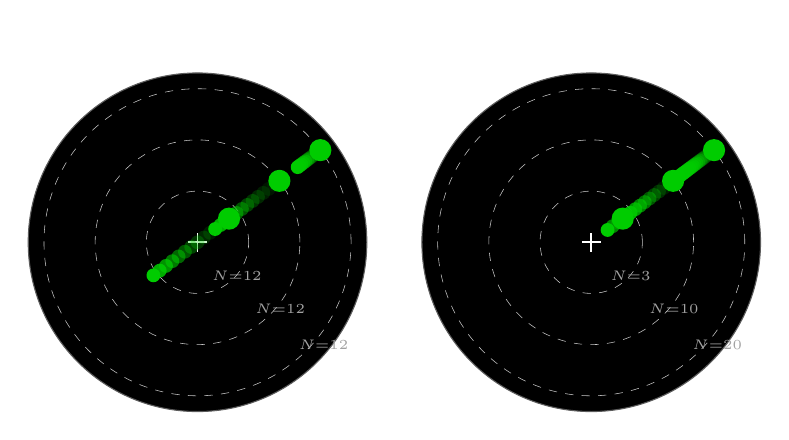
\begin{tikzpicture}

% ============================================================
% PANEL (a): Fixed trail length N=12
% Center at (0, 0), radius 2.0cm
% ============================================================

% Title
\node[white, font=\small\bfseries] at (0, 2.45) {(a) Fixed trail ($N=12$)};

% Black background circle
\fill[black] (0,0) circle (2.15cm);
\draw[Black70, line width=0.4pt] (0,0) circle (2.15cm);

% Range rings: dashed, Black30, at 0.65, 1.3, 1.95 cm
\draw[Black30, dashed, very thin] (0,0) circle (0.65cm);
\draw[Black30, dashed, very thin] (0,0) circle (1.30cm);
\draw[Black30, dashed, very thin] (0,0) circle (1.95cm);

% Crosshair
\draw[white, line width=0.6pt] (-0.12,0) -- (0.12,0);
\draw[white, line width=0.6pt] (0,-0.12) -- (0,0.12);

% N=12 labels near rings
\node[Black50, font=\tiny] at (0.50,-0.42) {$N$=12};
\node[Black50, font=\tiny] at (1.05,-0.85) {$N$=12};
\node[Black50, font=\tiny] at (1.60,-1.30) {$N$=12};

% --- NEAR target (fixed N=12): too long streak, widely spaced
% Target at ~(0.40, 0.30), direction (0.8, 0.6), spacing 0.10cm
\foreach \i/\op in {1/0.06,2/0.10,3/0.15,4/0.20,5/0.26,6/0.33,7/0.41,8/0.50,9/0.60,10/0.72,11/0.85,12/1.0}{%
  \fill[RadarGreen, opacity=\op] ({0.40 - \i*0.8*0.10}, {0.30 - \i*0.6*0.10}) circle (2.5pt);
}
\fill[RadarGreen] (0.40, 0.30) circle (4pt);

% --- MID target (fixed N=12): moderate spacing
% Target at ~(1.04, 0.78), direction (0.8, 0.6), spacing 0.085cm
\foreach \i/\op in {1/0.06,2/0.10,3/0.15,4/0.20,5/0.26,6/0.33,7/0.41,8/0.50,9/0.60,10/0.72,11/0.85,12/1.0}{%
  \fill[RadarGreen, opacity=\op] ({1.04 - \i*0.8*0.085}, {0.78 - \i*0.6*0.085}) circle (2.5pt);
}
\fill[RadarGreen] (1.04, 0.78) circle (4pt);

% --- FAR target (fixed N=12): short effective displacement (0.030cm spacing)
% Target at ~(1.56, 1.17), direction (0.8, 0.6), spacing 0.030cm
\foreach \i/\op in {1/0.06,2/0.10,3/0.15,4/0.20,5/0.26,6/0.33,7/0.41,8/0.50,9/0.60,10/0.72,11/0.85,12/1.0}{%
  \fill[RadarGreen, opacity=\op] ({1.56 - \i*0.8*0.030}, {1.17 - \i*0.6*0.030}) circle (2.5pt);
}
\fill[RadarGreen] (1.56, 1.17) circle (4pt);

% ============================================================
% PANEL (b): Range-adaptive trail
% Center at (5.0, 0), radius 2.0cm
% ============================================================

\def\cx{5.0}

% Title
\node[white, font=\small\bfseries] at (\cx, 2.45) {(b) Range-adaptive trail};

% Black background circle
\fill[black] (\cx,0) circle (2.15cm);
\draw[Black70, line width=0.4pt] (\cx,0) circle (2.15cm);

% Range rings
\draw[Black30, dashed, very thin] (\cx,0) circle (0.65cm);
\draw[Black30, dashed, very thin] (\cx,0) circle (1.30cm);
\draw[Black30, dashed, very thin] (\cx,0) circle (1.95cm);

% Crosshair
\draw[white, line width=0.6pt] ({\cx-0.12},0) -- ({\cx+0.12},0);
\draw[white, line width=0.6pt] (\cx,-0.12) -- (\cx,0.12);

% N labels near rings
\node[Black50, font=\tiny] at ({\cx+0.50},-0.42) {$N$=3};
\node[Black50, font=\tiny] at ({\cx+1.05},-0.85) {$N$=10};
\node[Black50, font=\tiny] at ({\cx+1.60},-1.30) {$N$=20};

% --- NEAR target (adaptive N=3): short clean trail, 3 dots at wide spacing
% Target at ~(cx+0.40, 0.30), direction (0.8, 0.6), spacing 0.08cm (compact)
\foreach \i/\op in {1/0.30,2/0.65,3/1.0}{%
  \fill[RadarGreen, opacity=\op] ({\cx+0.40 - \i*0.8*0.08}, {0.30 - \i*0.6*0.08}) circle (2.5pt);
}
\fill[RadarGreen] ({\cx+0.40}, 0.30) circle (4pt);

% --- MID target (adaptive N=10): medium trail
% Target at ~(cx+1.04, 0.78), direction (0.8, 0.6), spacing 0.075cm
\foreach \i/\op in {1/0.07,2/0.14,3/0.22,4/0.31,5/0.41,6/0.52,7/0.63,8/0.74,9/0.87,10/1.0}{%
  \fill[RadarGreen, opacity=\op] ({\cx+1.04 - \i*0.8*0.075}, {0.78 - \i*0.6*0.075}) circle (2.5pt);
}
\fill[RadarGreen] ({\cx+1.04}, 0.78) circle (4pt);

% --- FAR target (adaptive N=20): long trail, closely spaced dots to build up signal
% Target at ~(cx+1.56, 1.17), direction (0.8, 0.6), spacing 0.028cm
\foreach \i/\op in {1/0.04,2/0.07,3/0.10,4/0.14,5/0.18,6/0.23,7/0.28,8/0.33,9/0.39,10/0.45,11/0.51,12/0.57,13/0.63,14/0.69,15/0.75,16/0.80,17/0.86,18/0.91,19/0.96,20/1.0}{%
  \fill[RadarGreen, opacity=\op] ({\cx+1.56 - \i*0.8*0.028}, {1.17 - \i*0.6*0.028}) circle (2.5pt);
}
\fill[RadarGreen] ({\cx+1.56}, 1.17) circle (4pt);

\end{tikzpicture}
\end{document}
